\documentclass[Deriaz_Traiber_Labo02.tex]{subfiles}


\begin{document}
\chapter{Antenne patch}
\section{Objectif}
Le but est de réaliser une antenne qui résonne autour de \SI{1.575}{\giga\hertz}. On mesure le $s_{11}$ pour déterminer la bande passante. Le but est d'obtenir \SI{-10}{\deci\bel} sur une largeur de bande de \SI{40}{\mega\hertz}.

\begin{figure}[H]
\centering
\includegraphics[scale=1,page=2]{../Schemas-crop.pdf}
\caption{Dimensions de l'antenne patch}
\end{figure}
\begin{table}[H]
\centering
\begin{tabular}{lll}
\textbf{Variables}\\\hline
$w_0$ & Largeur du pied\\
$w_1$ & Espacement entre le pied et l'antenne\\
$y_1$ & Hauteur du pied à l'extérieur de l'antenne\\
$y_0$ & Hauteur du pied à l'intérieur de l'antenne\\
$W$ & Longueur de l'antenne\\
$L$ & Largeur de l'antenne\\
\textbf{Constantes} & & \textbf{Valeur}\\\hline
$w_s$ & largeur du PCB & \SI{100}{\milli\meter}\\
$l_s$ & Longueur du PCB & \SI{100}{\milli\meter}\\
$h$ & Épaisseur du PCB & \SI{1.6}{\milli\meter}\\
$e$ & Épaisseur de cuivre & \SI{35}{\micro\meter}
\end{tabular}
\caption{Liste des dimensions}
\end{table}


\section{FR-4}
La valeur de $\epsilon_r$ pour le FR-4 est de 4.3
\subsection{Calculs}
La longueur $W$ est donnée par
$$W=\frac{1}{2f_r\sqrt{\epsilon_0\epsilon_r}}\sqrt{\frac{2}{\epsilon_r+1}}=\frac{c}{2f_r}\sqrt{\frac{2}{\epsilon_r+1}}$$
Avec $f_r=\SI{1.575}{\giga\hertz}$, on a la valeur suivante pour $W$
$$W=\SI{58.46}{\milli\meter}$$
La valeur de $\epsilon_{reff}$ permet de calculer les valeurs suivantes et est donnée par
$$\epsilon_{reff}=\frac{\epsilon_r+1}{2}+\frac{\epsilon_r-1}{2}\frac{1}{\sqrt{1+10\frac{h}{W}}}$$
La valeur de $\epsilon_{reff}$ calculée est la suivante
$$\epsilon_{reff}=4.11$$
La valeur $\Delta L$ est calculée de la manière suivante
$$\Delta L=0.412h\frac{\epsilon_r+0.3}{\epsilon_r-0.258}\cdot\frac{\frac{W}{h}+0.264}{\frac{W}{h}+0.8}$$
On obtient la valeur suivante
$$\Delta L=\SI{0.739}{\milli\meter}$$
La valeur de $L$ se calcule de la manière suivante
$$L=\frac{1}{2f_r\sqrt{\epsilon_r\mu_0}}\sqrt{\frac{1}{\epsilon_{reff}-2\Delta L}}$$
La valeur calculée de $L$ est
$$L=\SI{46.94}{\milli\meter}$$
$Z_{in}$ est calculée avec
$$Z_{in}=\frac{60}{\sqrt{\epsilon_{reff}}}\ln\left(\frac{8h}{w_0}+\frac{w_0}{4h}\right)$$
L'objectif est d'atteindre $Z_{in}=\SI{50}{\ohm}$. Ce n'est pas possible car le fonction ne passe pas par ce point, mais il est possible de choisir le point le plus proche, soit
$$w_0=\SI{1.59}{\milli\meter}$$
\begin{figure}[H]
\centering
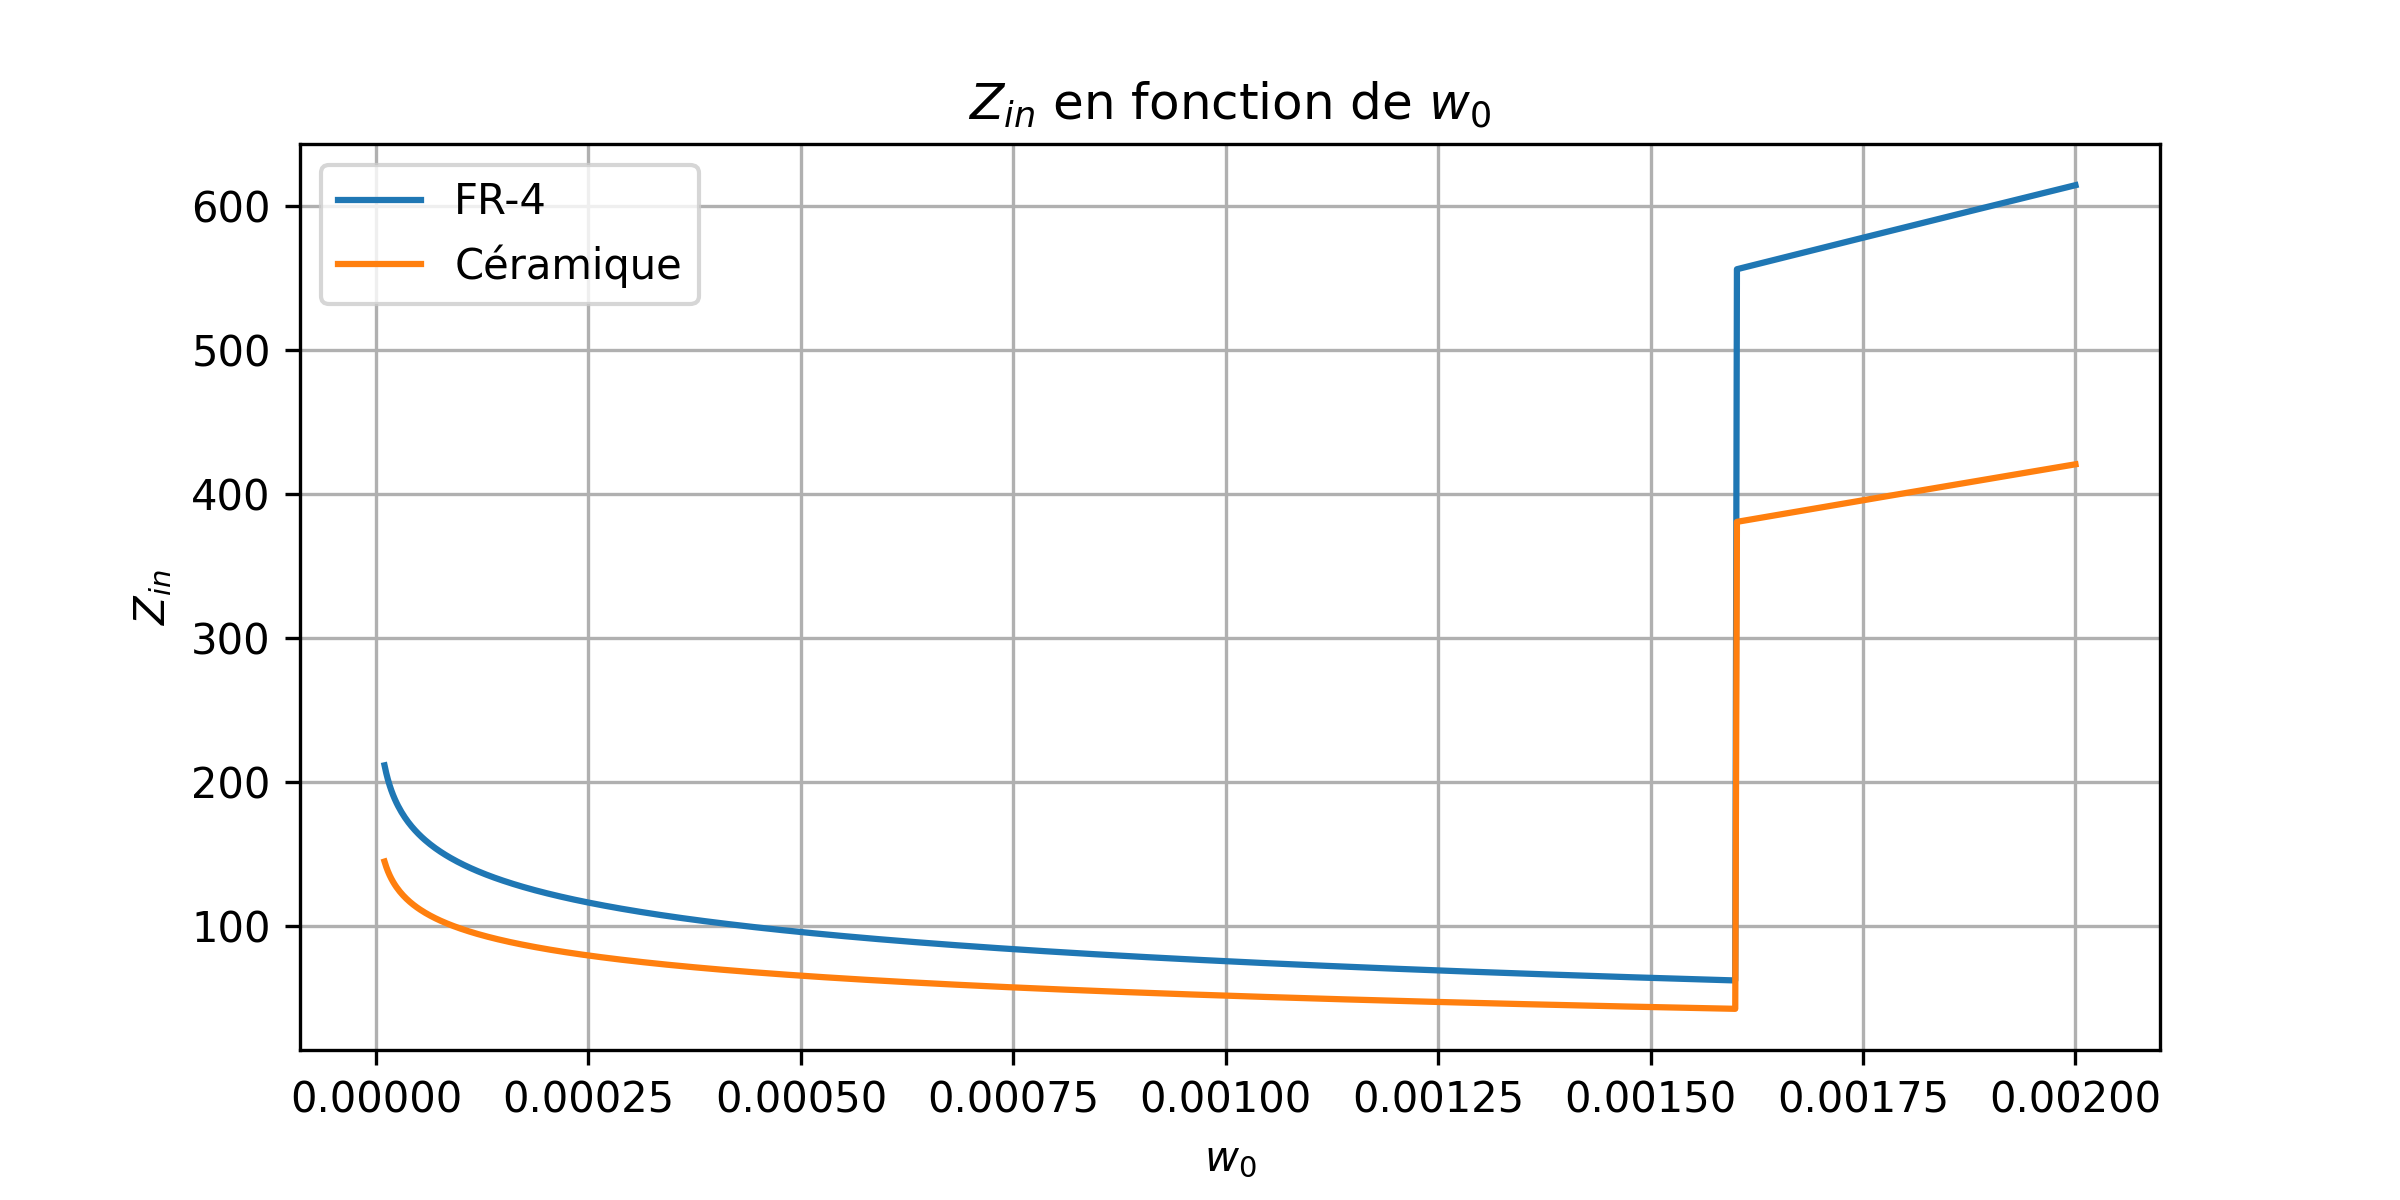
\includegraphics[width=12cm]{../Calculs/w0.png}
\caption{Impédance $Z_{in}$ en fonction de $w_0$}
\end{figure}
La distance $y_1$ est calculée en faisant
$$y_1=\frac{c}{8f_r}$$
Soit
$$y_1=\SI{23.79}{\milli\meter}$$
\subsection{Itérations}
\subsubsection{Première itération}
La première itération (avec les valeurs calculées) donne :
\begin{figure}[H]
\centering
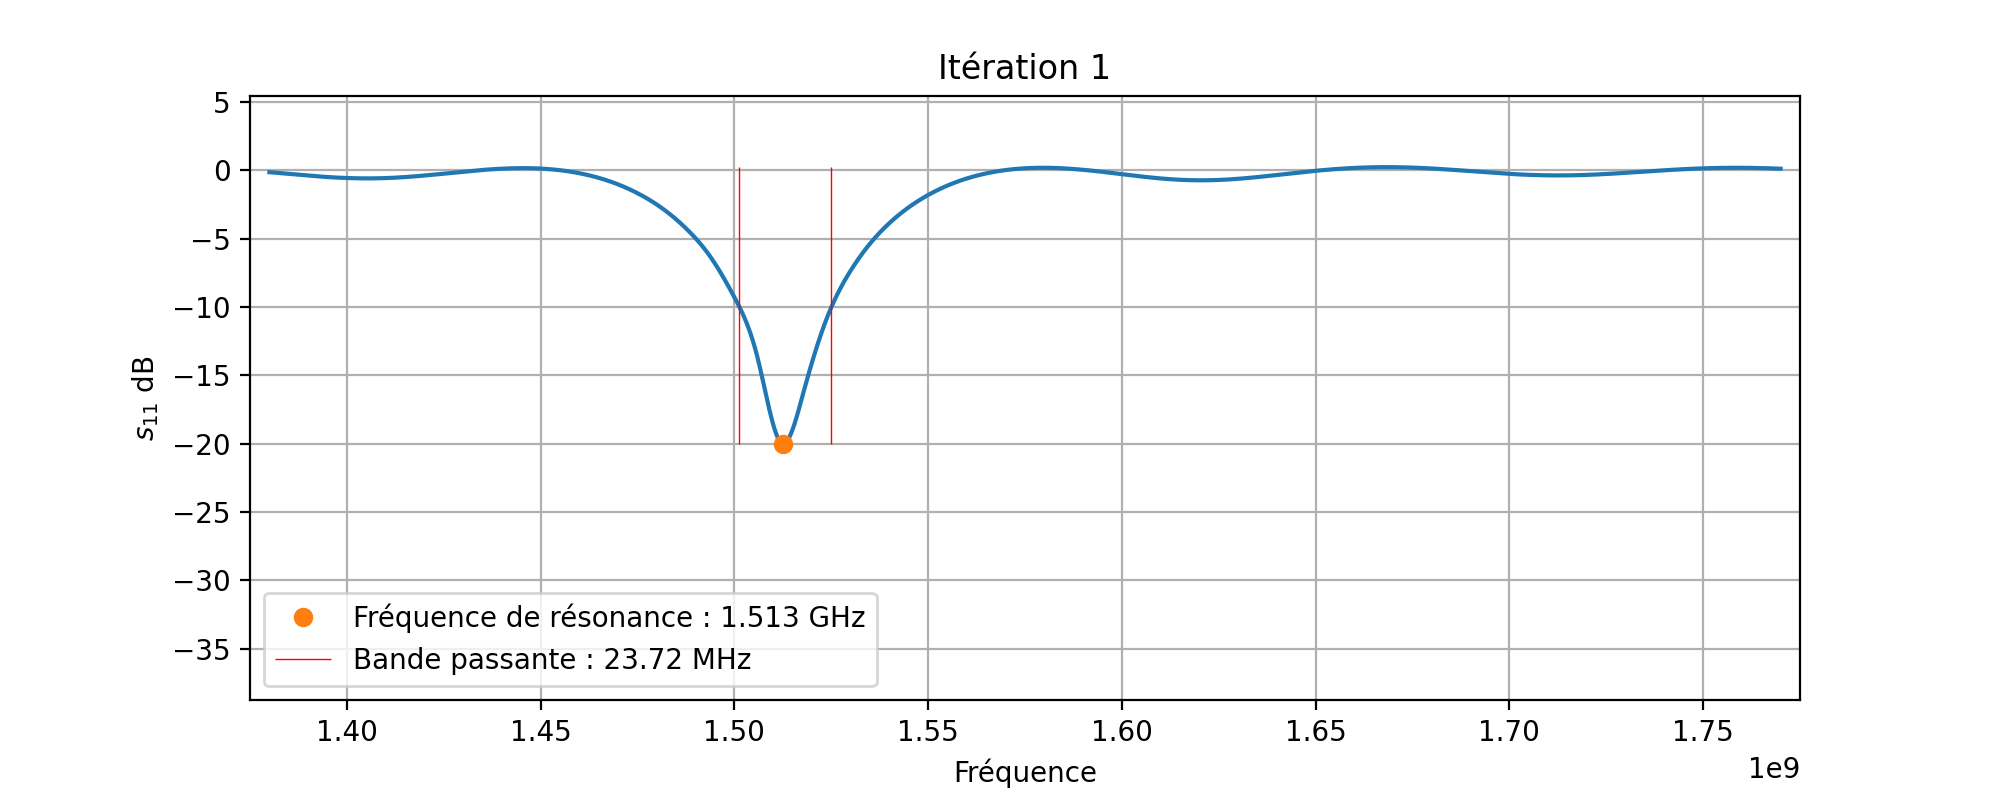
\includegraphics[width=15cm]{../Calculs/run_id_fr4_1.png}
\caption[caption]{$s_{11}$ de la première itération}
\end{figure}
La fréquence de résonance n'est pas bonne, pour l'ajuster nous avons choisi d'effectuer une règle de trois sur les dimensions de la patch ($W$ et $L$)
$$W'=\frac{1.513}{1.575}\cdot \SI{58.46}{\milli\meter}=\SI{56.16}{\milli\meter}$$
$$L'=\frac{1.513}{1.575}\cdot \SI{46.9}{\milli\meter}=\SI{45.05}{\milli\meter}$$
\subsubsection{Deuxième itération : correction de la fréquence de résonance}
\begin{figure}[H]
\centering
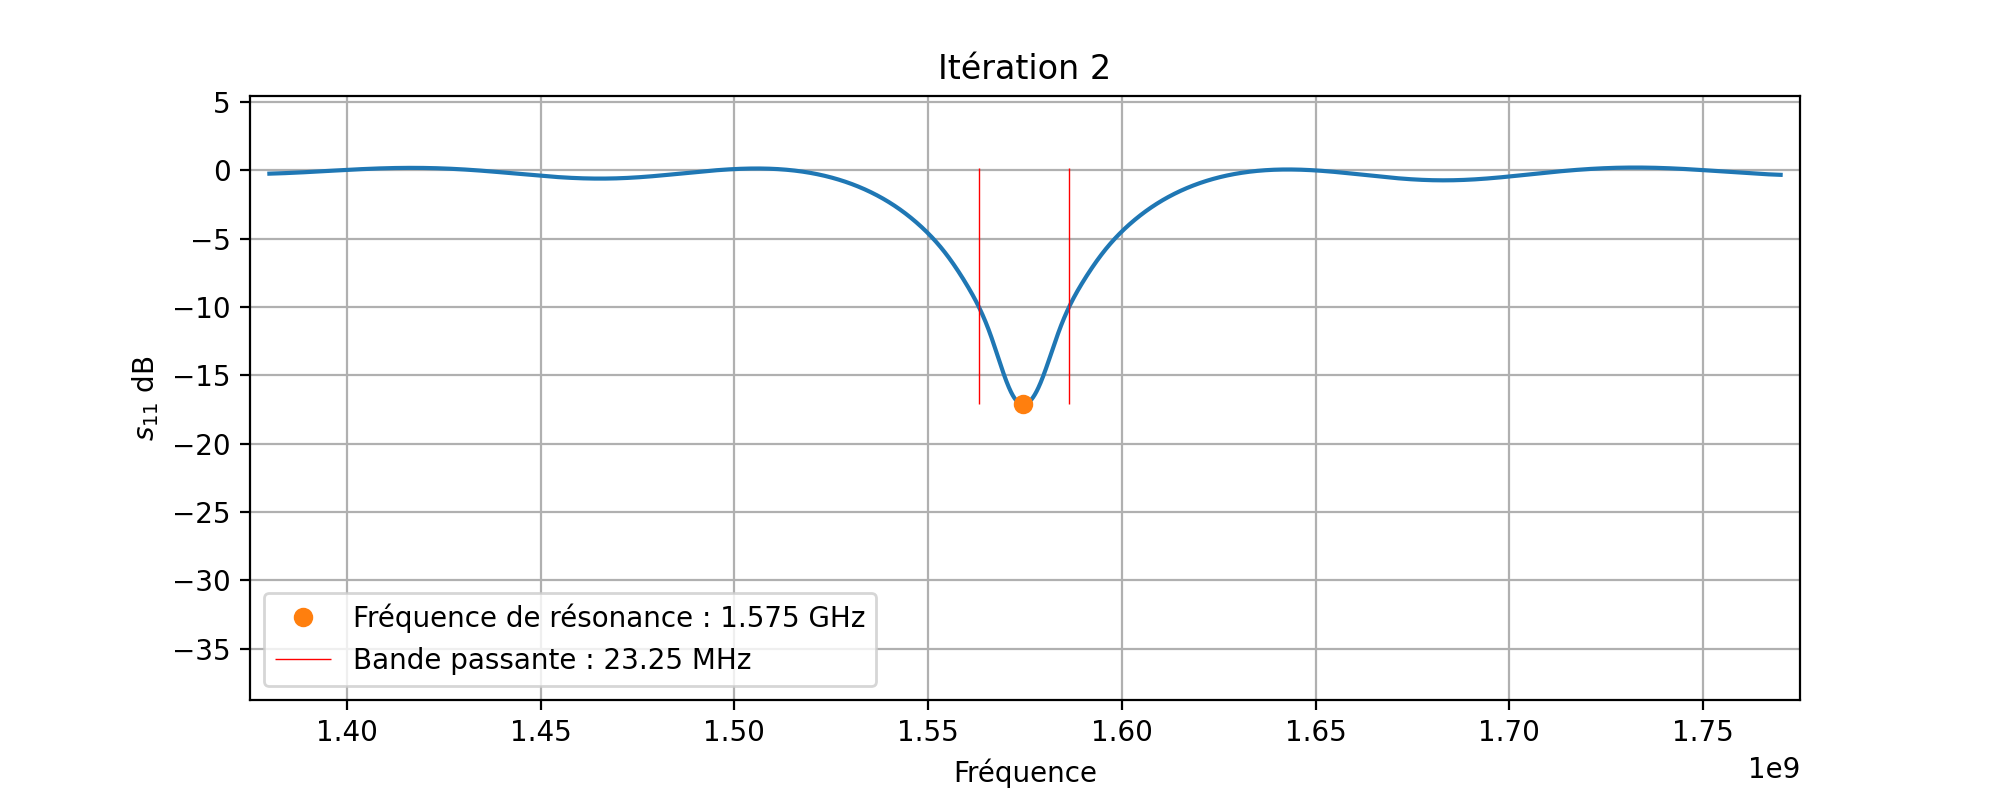
\includegraphics[width=15cm]{../Calculs/run_id_fr4_2.png}
\caption[caption]{$s_{11}$ de la deuxième itération}
\end{figure}
La fréquence est parfaitement celle que l'on cherche. La règle de trois est une bonne approximation. Il reste toutefois à augmenter la bande passante
\subsubsection{Troisième itération : Essai d'augmentation de la bande passante}
Nous avons essayé de modifier la taille de $y_0$ en la passant de \SI{14}{\milli\meter} à \SI{10}{\milli\meter}
\begin{figure}[H]
\centering
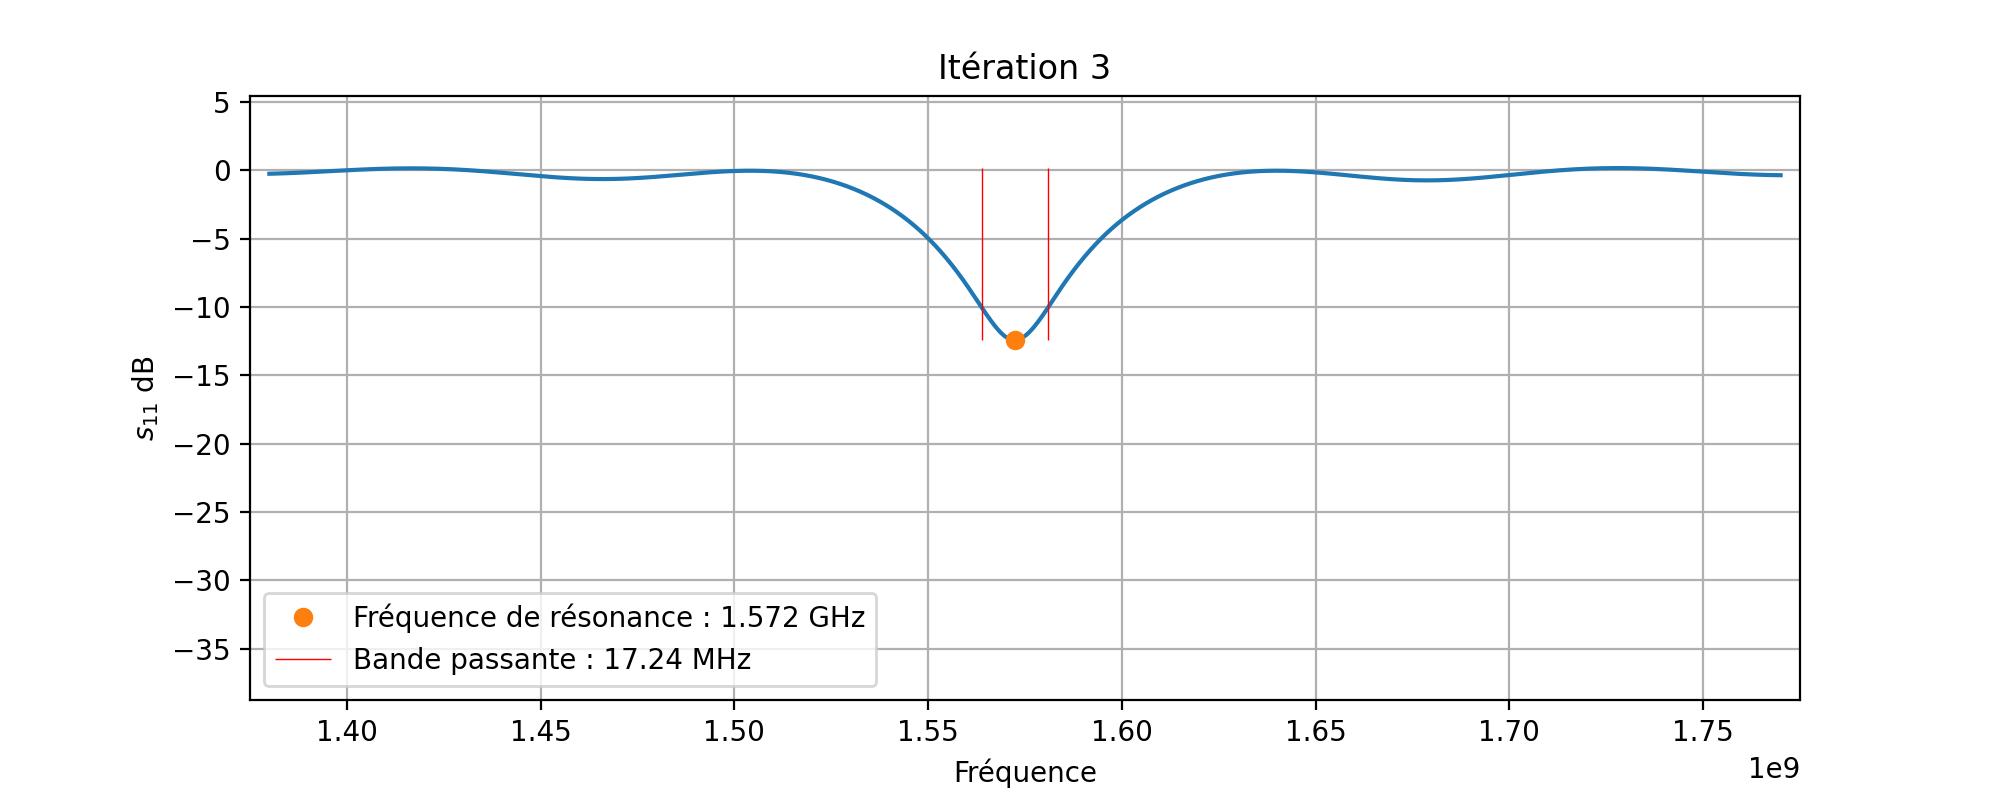
\includegraphics[width=15cm]{../Calculs/run_id_fr4_3.png}
\caption[caption]{$s_{11}$ de la troisième itération}
\end{figure}
La bande passante est plus mauvaise
\subsubsection{Quatrième itération : Essai d'augmentation de la bande passante}
Nous avons essayé de re-modifier $y_0$ en passant de \SI{10}{\milli\meter} à \SI{25}{\milli\meter}
\begin{figure}[H]
\centering
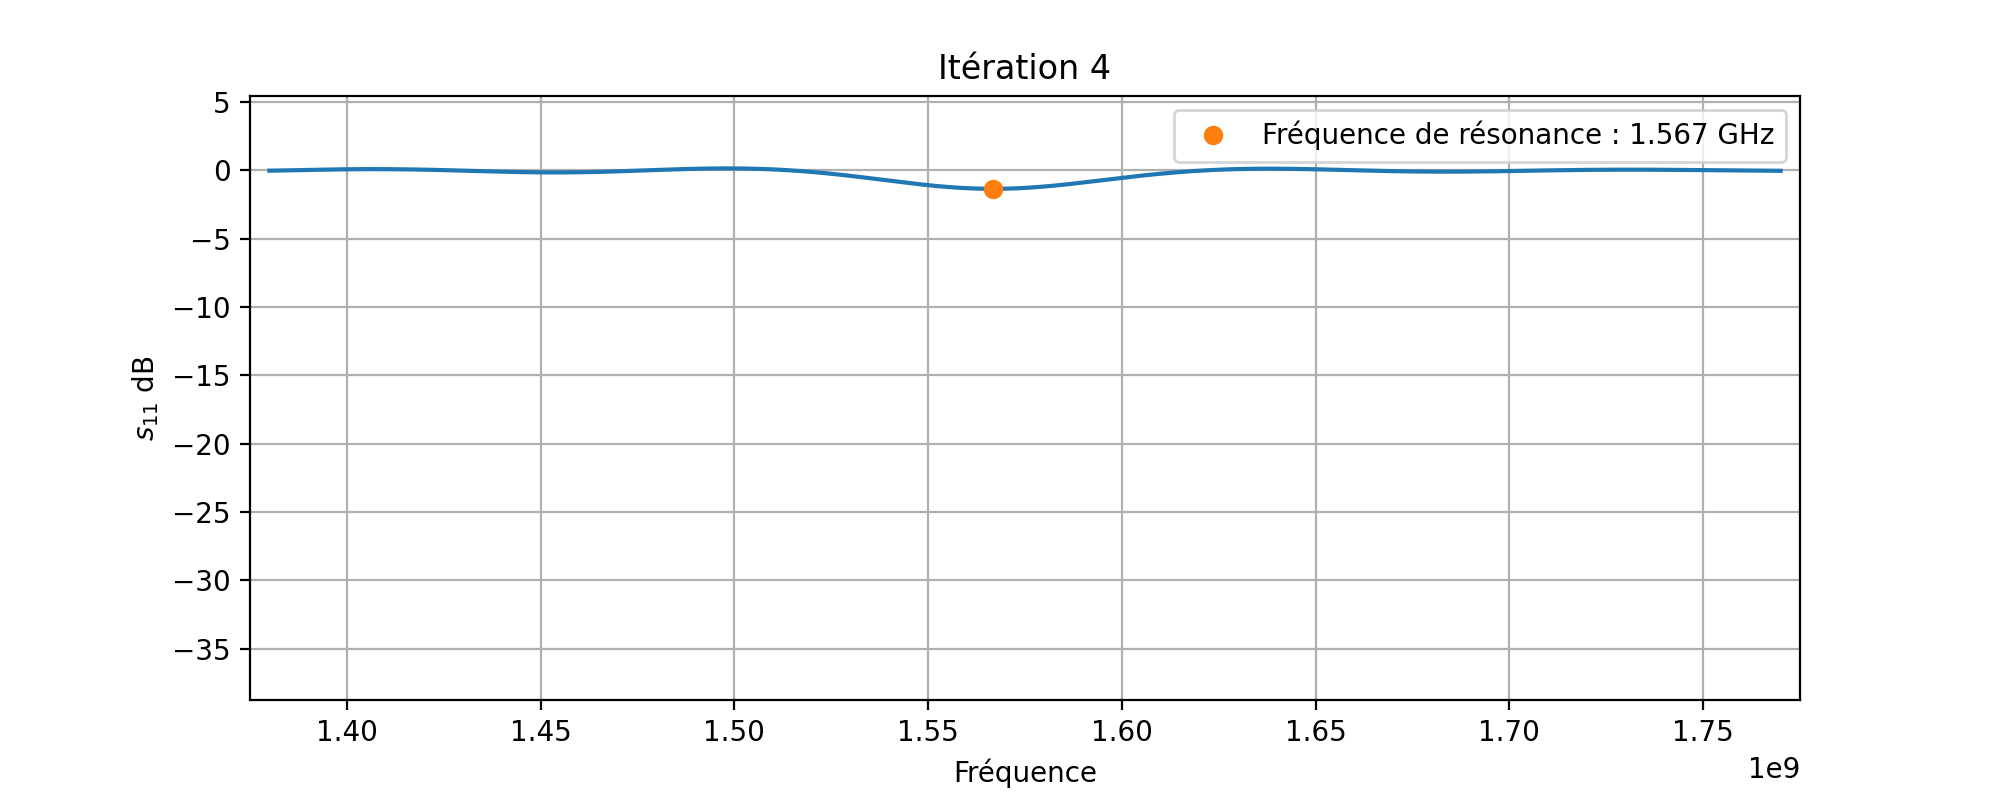
\includegraphics[width=15cm]{../Calculs/run_id_fr4_4.png}
\caption[caption]{$s_{11}$ de la quatrième itération}
\end{figure}
Pratiquement plus aucune résonance, la modification était trop importante.
\subsubsection{Cinquième itération : Essai d'augmentation de la bande passante}
Nous avons repris une valeur proche du départ pour $y_0$, soit \SI{16}{\milli\meter} et changé la valeur de $y_1$, soit \SI{18}{\milli\meter} au lieu de \SI{23.8}{\milli\meter}
\begin{figure}[H]
\centering
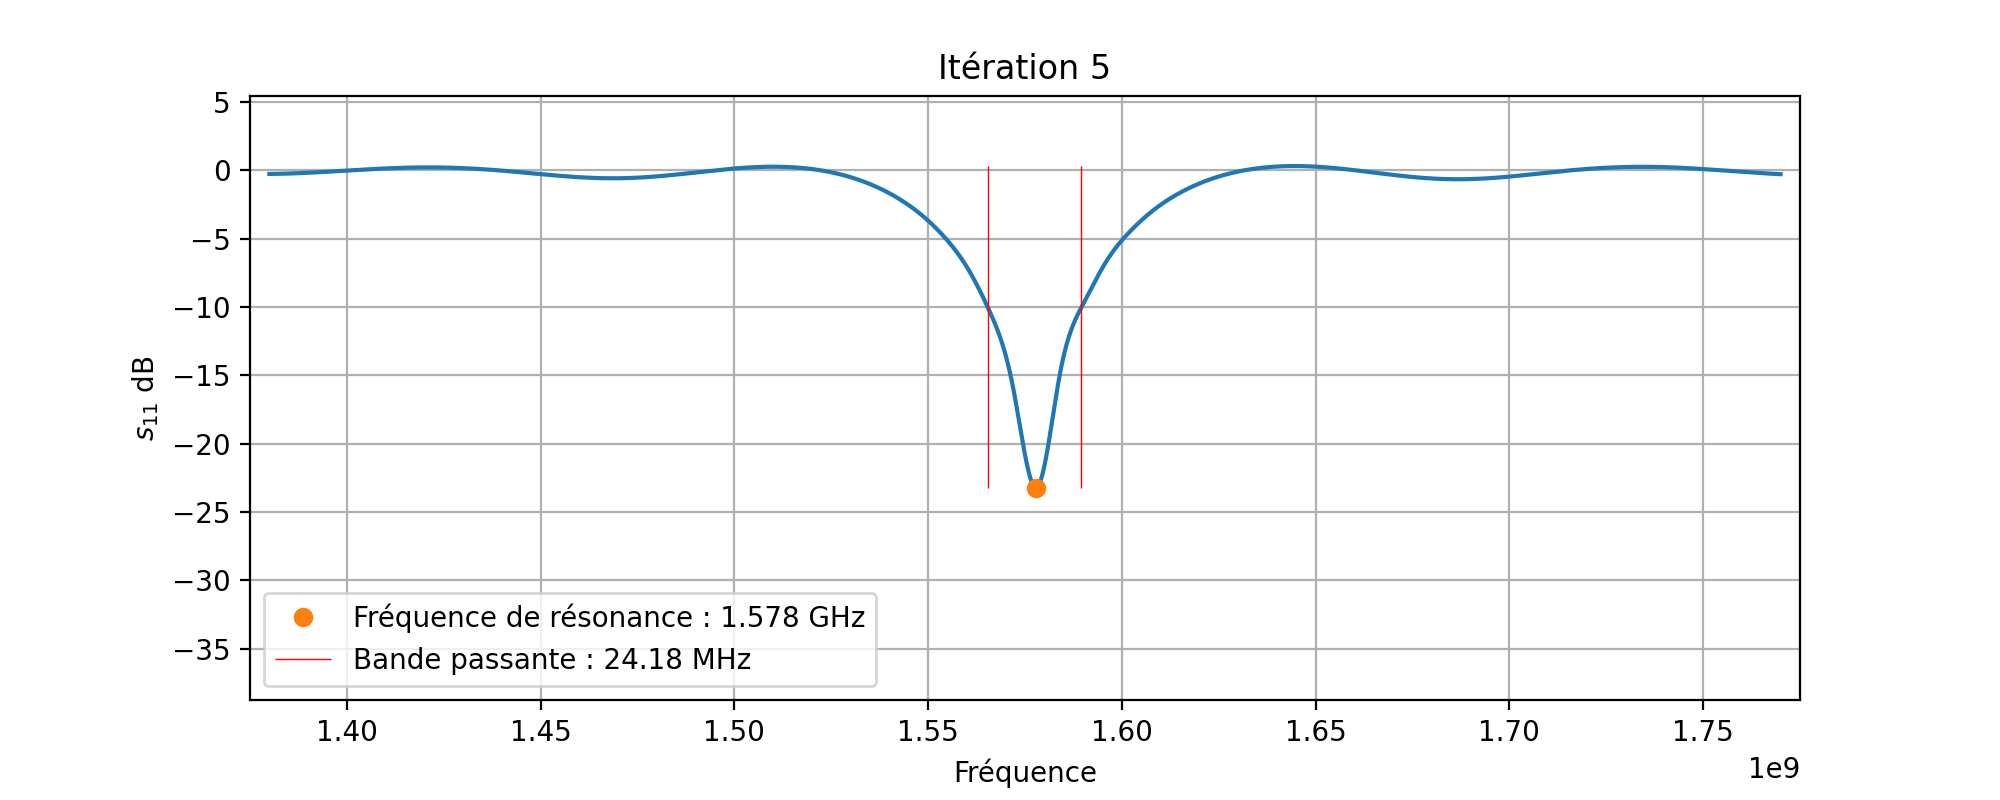
\includegraphics[width=15cm]{../Calculs/run_id_fr4_5.png}
\caption[caption]{$s_{11}$ de la cinquième itération}
\end{figure}
La bande passante est un peu meilleure, mais de très peu. La fréquence de résonance est plus basse en revanche (\SI{-23}{\deci\bel} au lieu de \SI{-17}{\deci\bel} dans l'itération deux).
\subsubsection{Itérations 6,7 et 8 : Tests en modifiant $w_0$ et $w_1$}
Toutes les modifications sur $w_0$ et $w_1$ n'ont montré aucune améliorations
\begin{figure}[H]
\centering
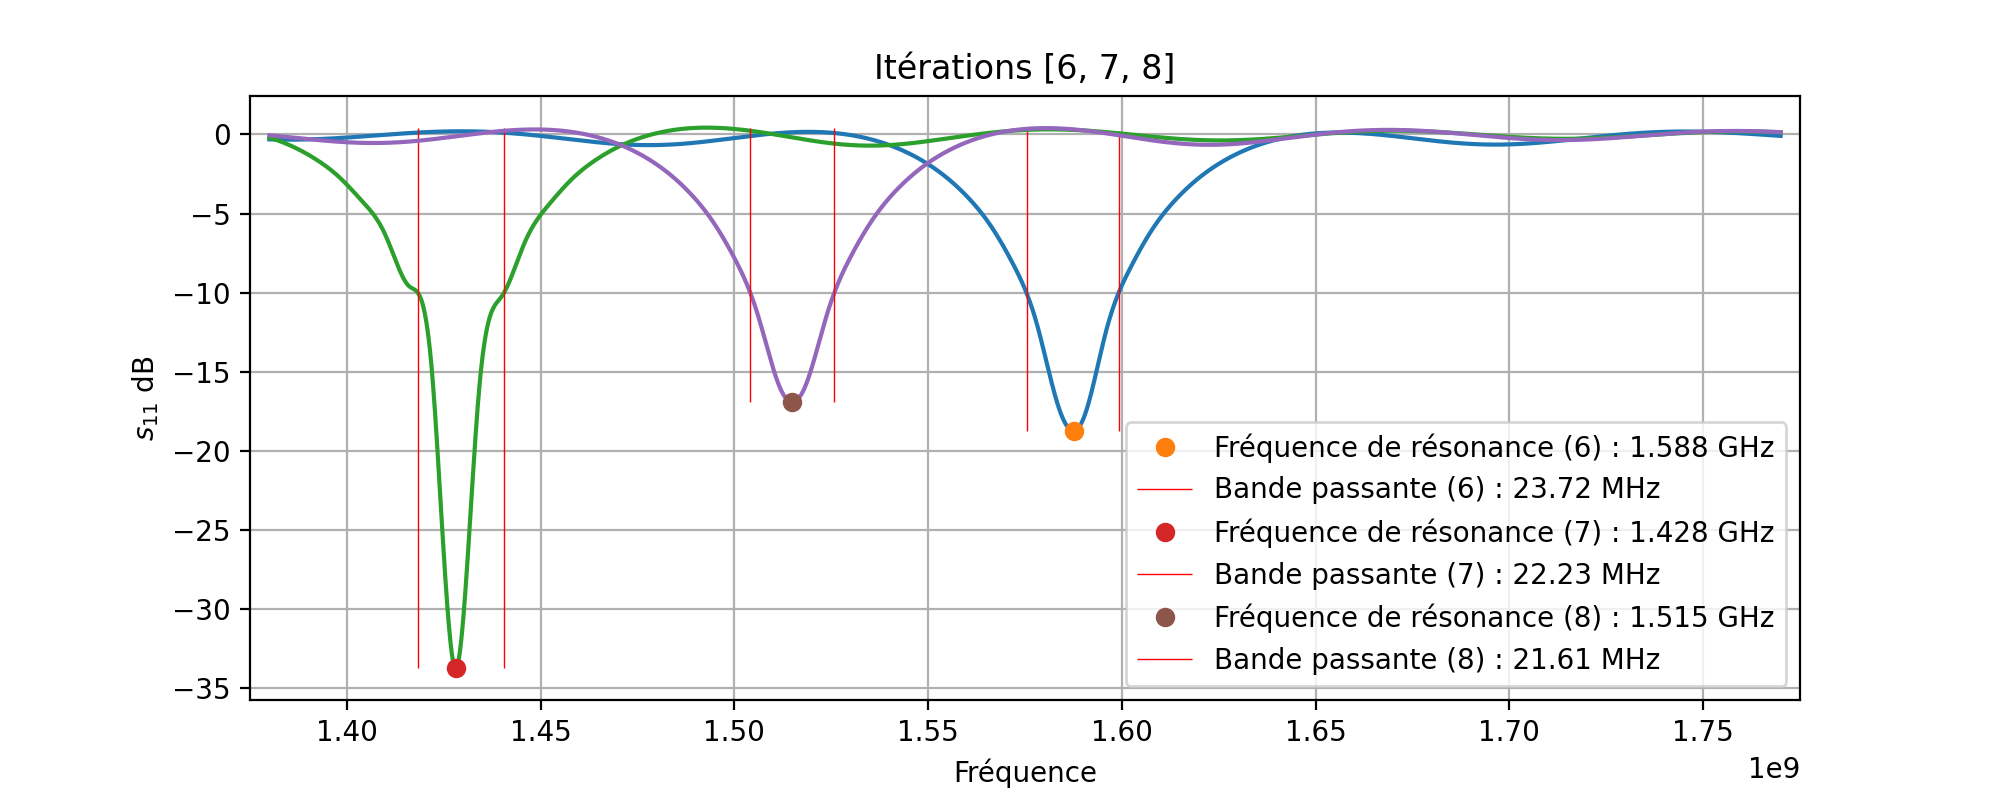
\includegraphics[width=15cm]{../Calculs/run_id_fr4_678.png}
\caption[caption]{$s_{11}$ des itérations 6,7,8}
\end{figure}
Les résultats sont mauvaise, nous avons repris les valeurs de l'itération 5
\subsubsection{Itération 9}
Les données sont celles de l'itération 5. La fréquence de résonance n'est pas parfaite
\subsubsection{Itération 10}
Correction de la fréquence de résonance par la règle de trois
\begin{figure}[H]
\centering
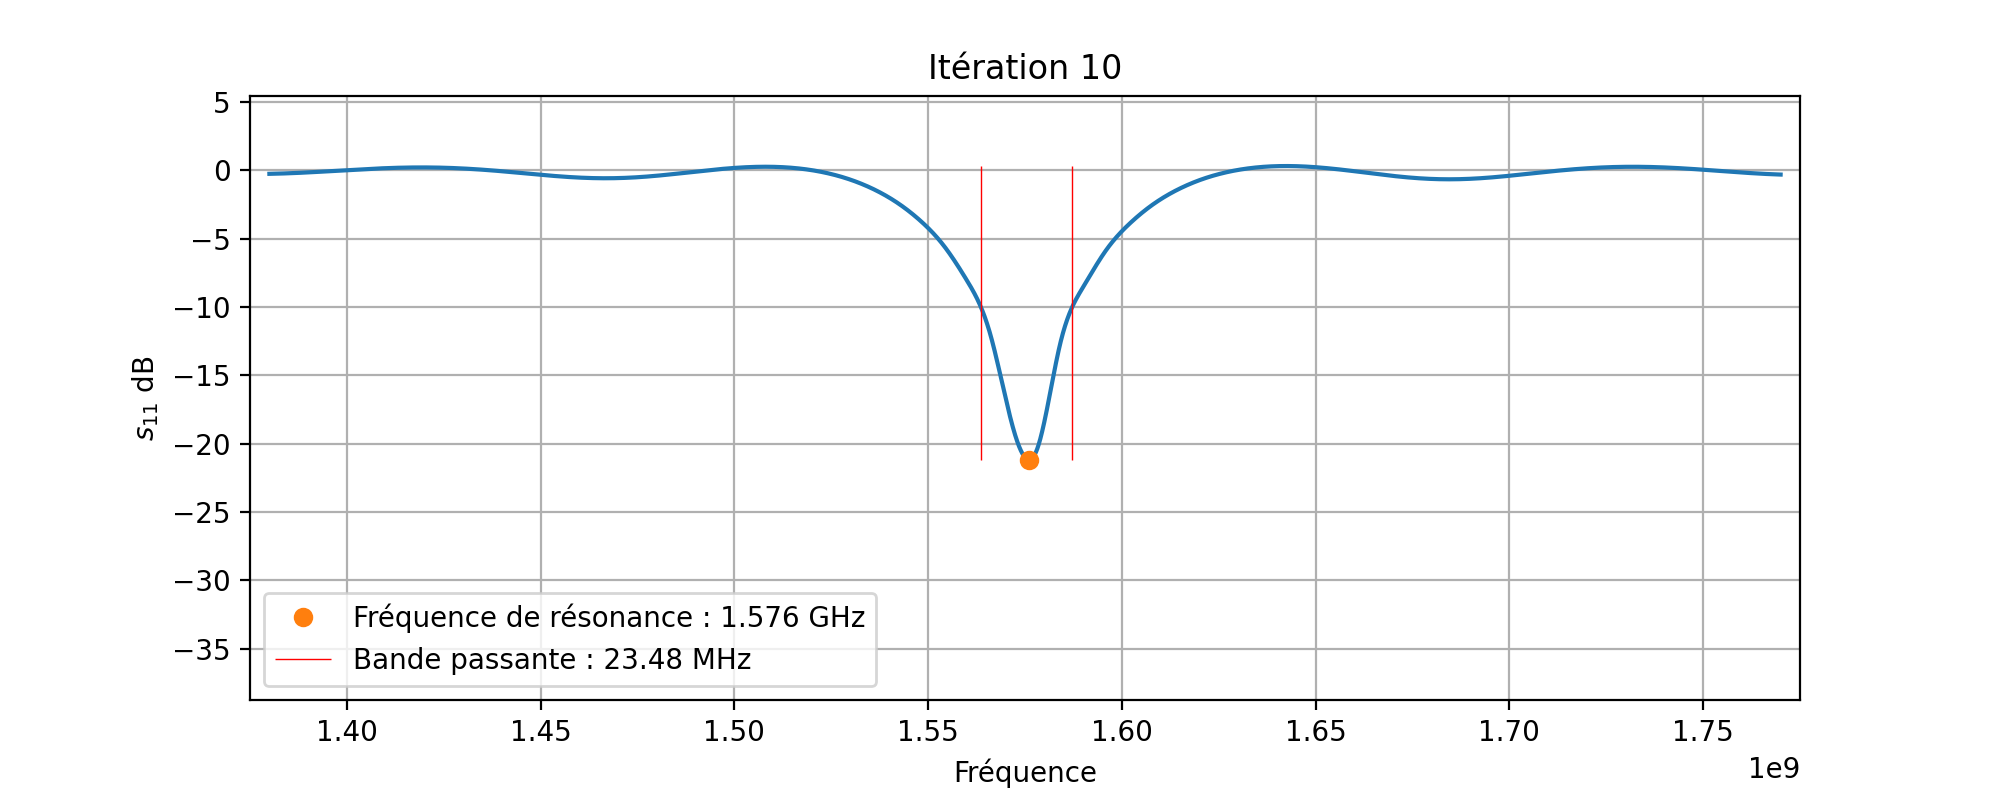
\includegraphics[width=15cm]{../Calculs/run_id_fr4_10.png}
\caption[caption]{$s_{11}$ de l'itération 10}
\end{figure}
La fréquence de résonance est acceptable. La bande passante n'est pas très bonne mais aucun paramètre modifiable ne semble la changer.
\subsubsection{Itérations 11 et 12 : test en modifiant l'épaisseur du circuit}
L'épaisseur a été modifiée à \SI{2.5}{\milli\meter} puis \SI{5}{\milli\meter}
\begin{figure}[H]
\centering
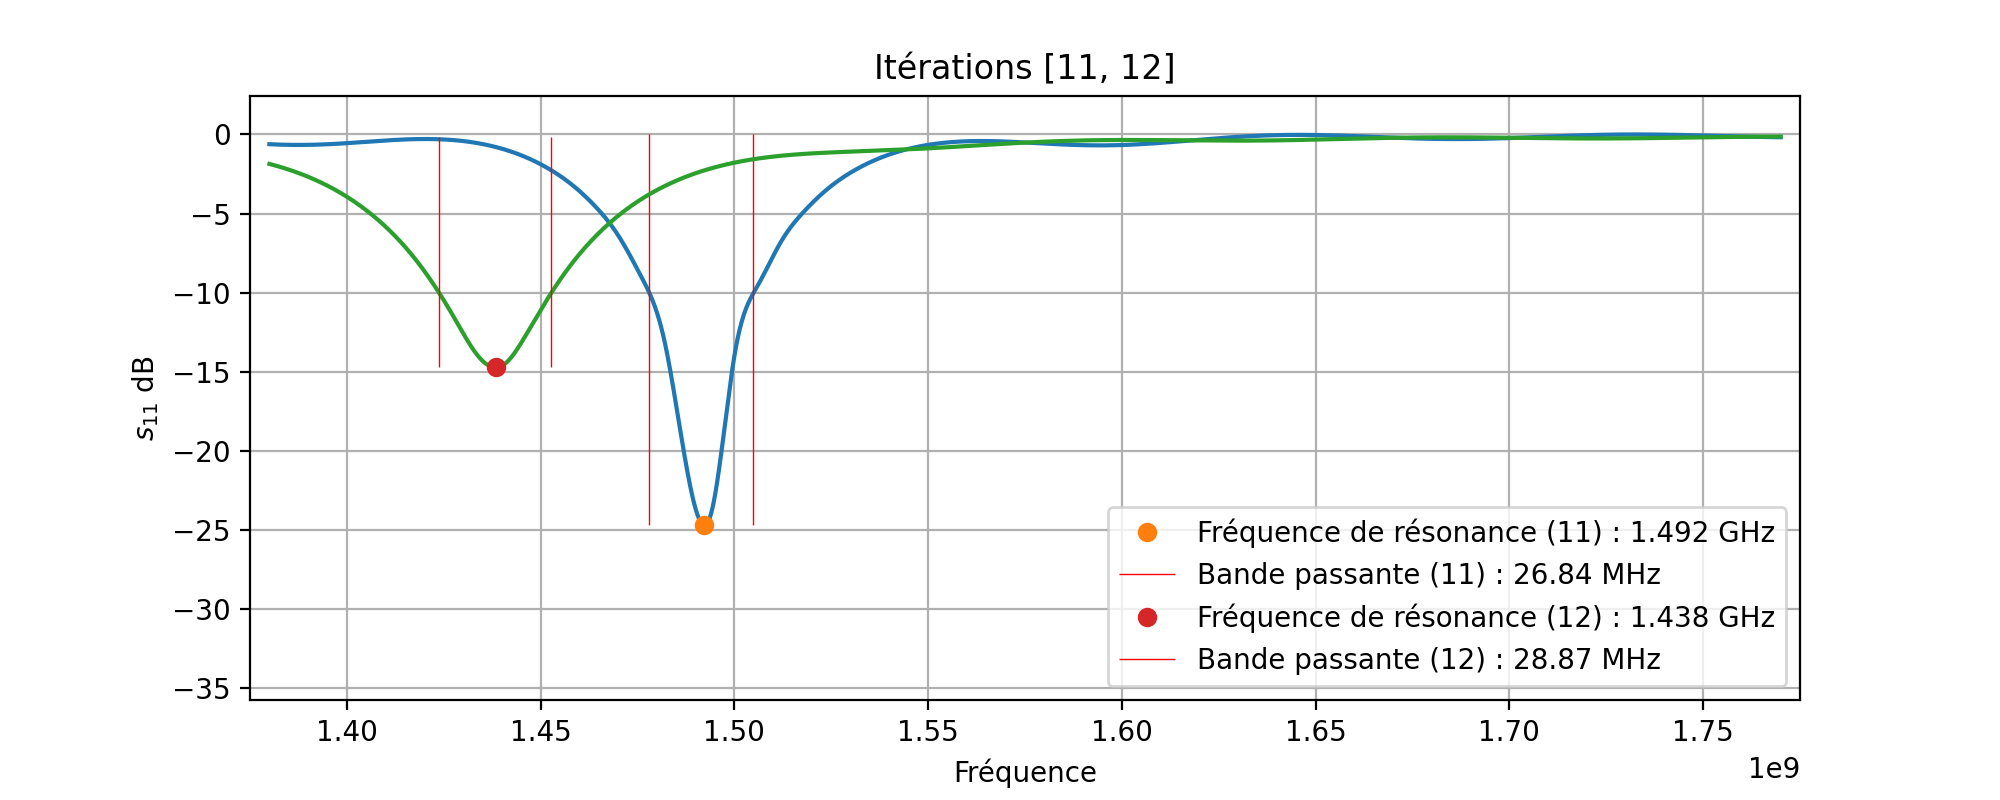
\includegraphics[width=15cm]{../Calculs/run_id_fr4_1112.png}
\caption[caption]{$s_{11}$ de l'itération 10}
\end{figure}
L'augmentation de l'épaisseur semble avoir un léger impact positif sur la bande passante.
\subsection{Conclusion}
La fréquence d'une antenne patch FR-4 peut facilement être ajustée en modifiant sa largeur et/ou sa longueur. Il est également possible d'obtenir un pic "profond" sur le $s_{11}$ en modifiant $y_0$ et $y_1$. En revanche il est très difficile, voir impossible de modifier la bande passante sans changer l'épaisseur du PCB.\\
Les dimensions finales sont
\begin{itemize}
\item $W=\SI{56.27}{\milli\meter}$
\item $L=\SI{45.08}{\milli\meter}$
\item $w_0=\SI{1.6}{\milli\meter}$
\item $y_1=\SI{18}{\milli\meter}$
\item $y_0=\SI{16}{\milli\meter}$
\end{itemize}
\section{Céramique}
La valeur de $\epsilon_r$ pour la céramique est de 4.3
\subsection{Calculs}
Les calculs sont les mêmes que pour l'antenne en FR-4, à l'exception d'un changement de $\epsilon_r$
\begin{itemize}
\item $W=\SI{41.7}{\milli\meter}$
\item $\epsilon_{reff}=8.77$
\item $\Delta L=\SI{0.685}{\milli\meter}$
\item $L=\SI{21.14}{\milli\meter}$
\item $w_0=\SI{1.1}{\milli\meter}$
\item $y_1=23.79$
\end{itemize}
\subsection{Itérations}
\subsubsection{Première itération}
Les valeurs sont celles calculées plus haut
\begin{figure}[H]
\centering
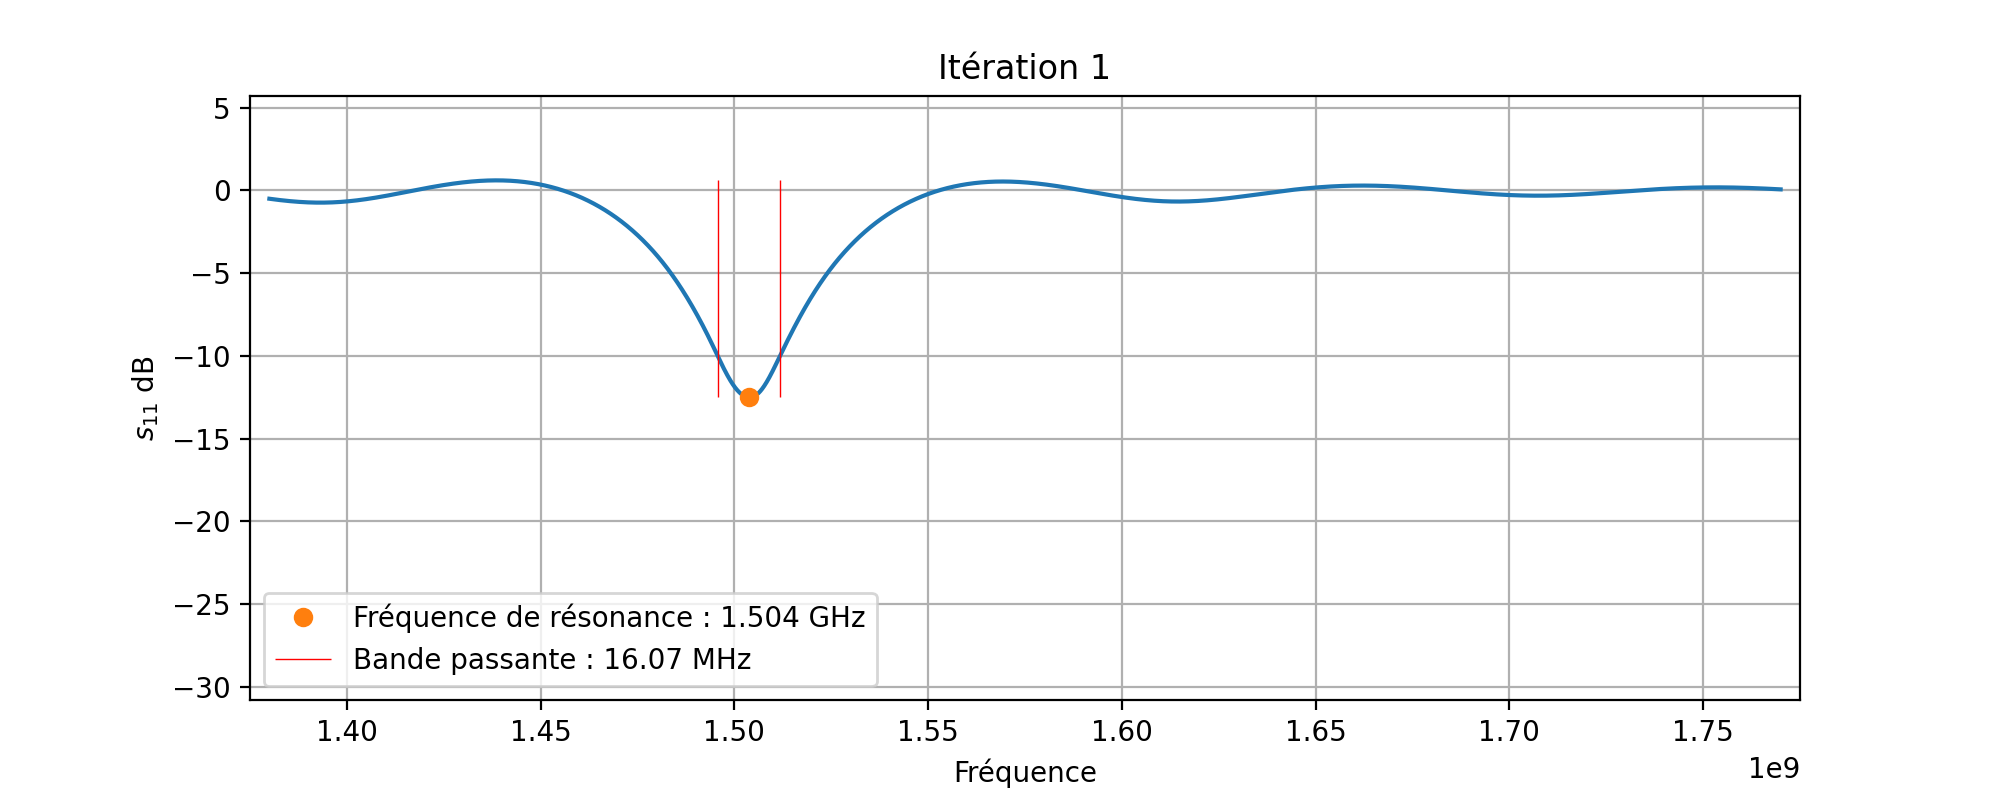
\includegraphics[width=15cm]{../Calculs/run_id_ceramique_1.png}
\caption[caption]{$s_{11}$ de l'itération 1}
\end{figure}
Le $s_{11}$ n'est pas très bon et la fréquence de résonance n'est pas bonne
\subsubsection{Deuxième itération : Amélioration du $s_{11}$}
Comme la fréquence est facile à modifier, nous avons augmenté le $y_0$ (à \SI{16}{\milli\meter}).
\begin{figure}[H]
\centering
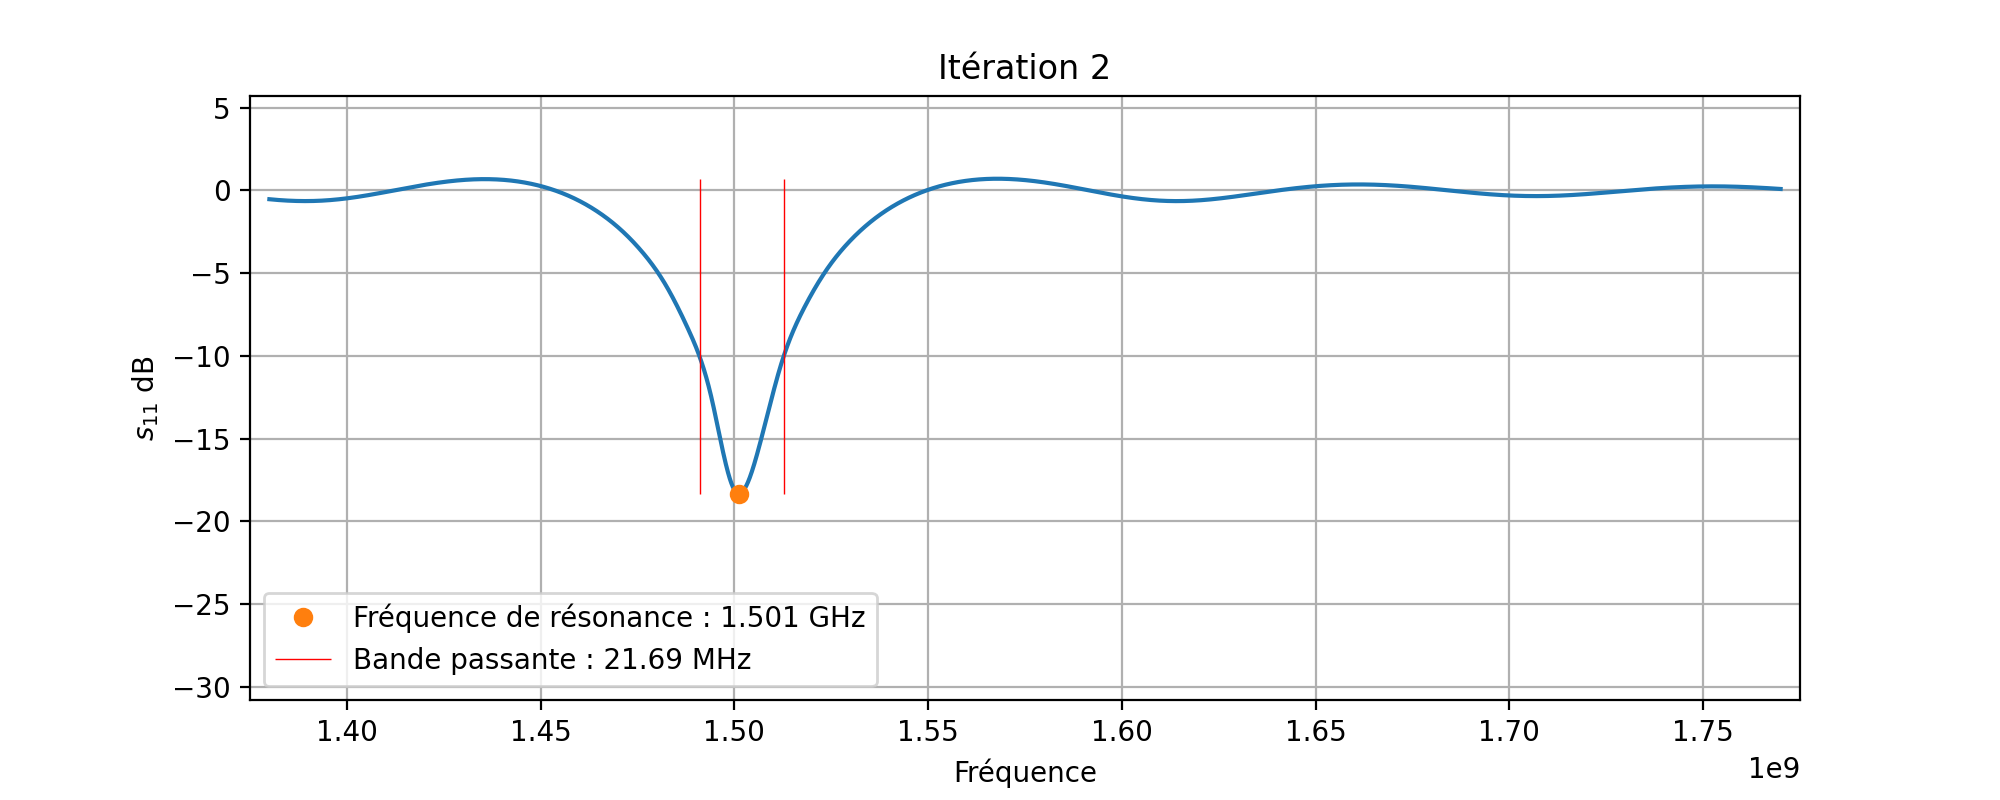
\includegraphics[width=15cm]{../Calculs/run_id_ceramique_2.png}
\caption[caption]{$s_{11}$ de l'itération 2}
\end{figure}
Le $s_{11}$ est meilleur
\subsubsection{Troisième itération : Amélioration du $s_{11}$}
L'étape précédente a fonctionner, nous recommençons avec $y_0=\SI{18}{\milli\meter}$
\begin{figure}[H]
\centering
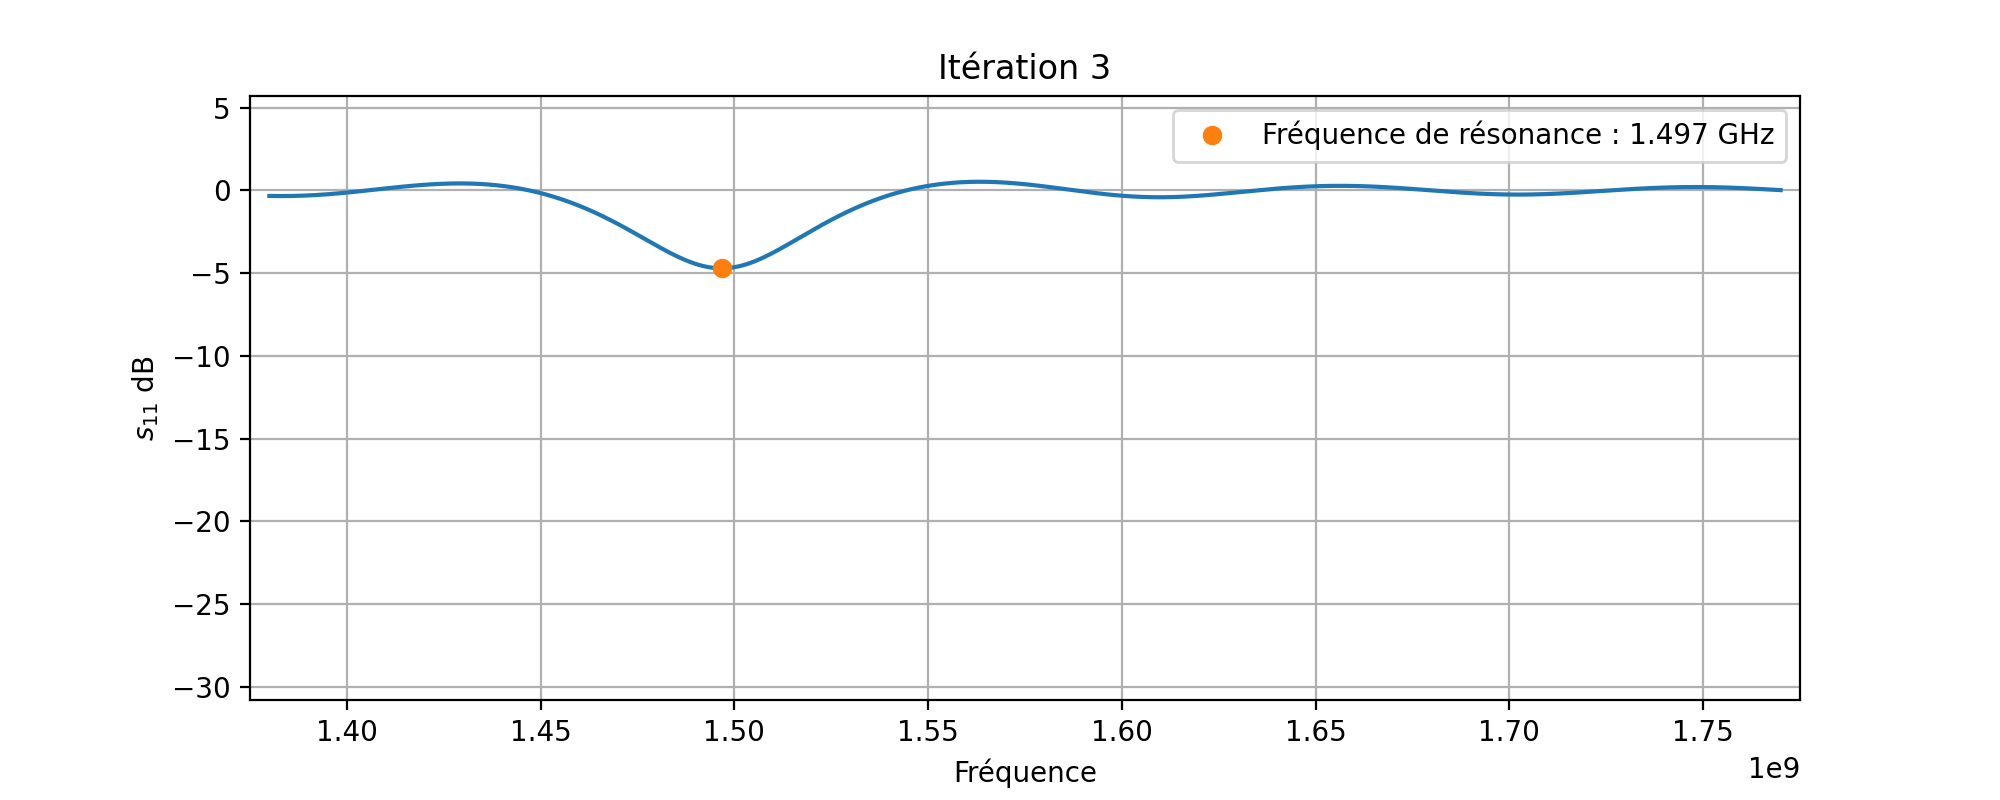
\includegraphics[width=15cm]{../Calculs/run_id_ceramique_3.png}
\caption[caption]{$s_{11}$ de l'itération 3}
\end{figure}
Le $s_{11}$ s'est grandement dégradé
\subsubsection{Quatrième itération : $y_0$ par régression}
Pour trouver le $y_0$, nous avons effectuée une régression quadratique sur les précédentes valeurs de $y_0$ (trois valeurs et trois valeurs minimales de $s_{11}$) pour trouver la valeur idéale de $y_0=\SI{15.4}{\milli\meter}$
\begin{figure}[H]
\centering
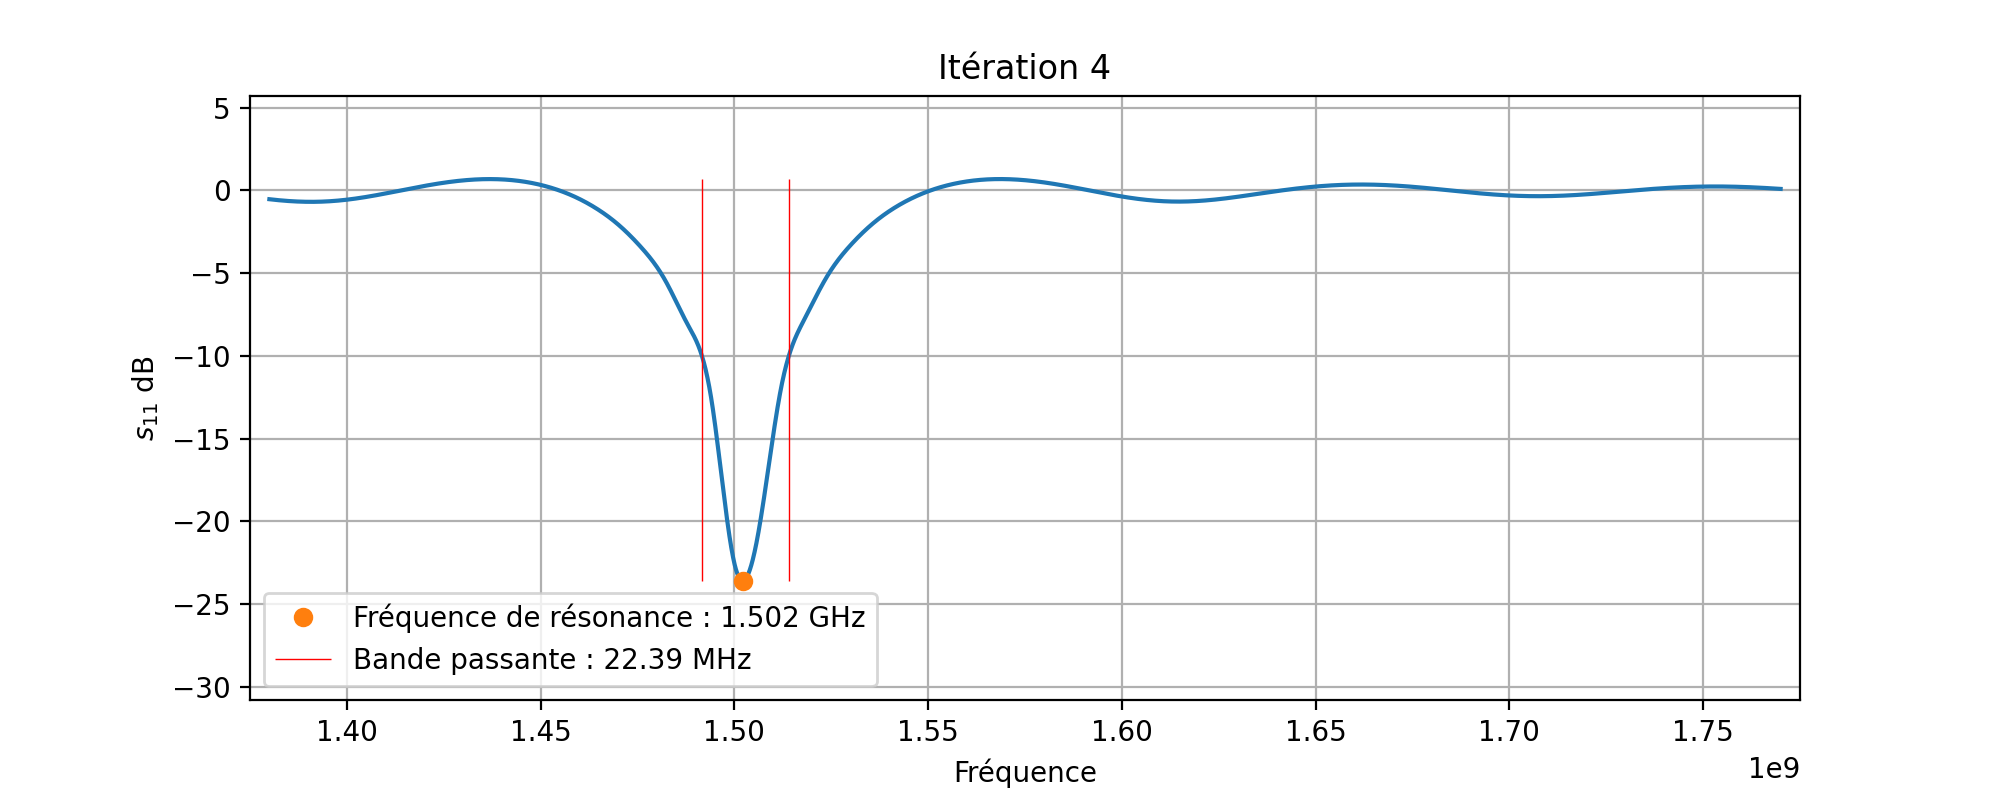
\includegraphics[width=15cm]{../Calculs/run_id_ceramique_4.png}
\caption[caption]{$s_{11}$ de l'itération 4}
\end{figure}
Le $s_{11}$ est très bas, comme on s'y attendait
\subsubsection{Cinquième itération : Correction de la fréquence de résonance}
Les nouveaux $W$ et $L$ sont trouvés par règle de 3
$$W'=\frac{1.502}{1.575}\cdot \SI{41.7}{\milli\meter}=\SI{39.77}{\milli\meter}$$
$$L'=\frac{1.502}{1.575}\cdot \SI{32.1}{\milli\meter}=\SI{30.61}{\milli\meter}$$
\begin{figure}[H]
\centering
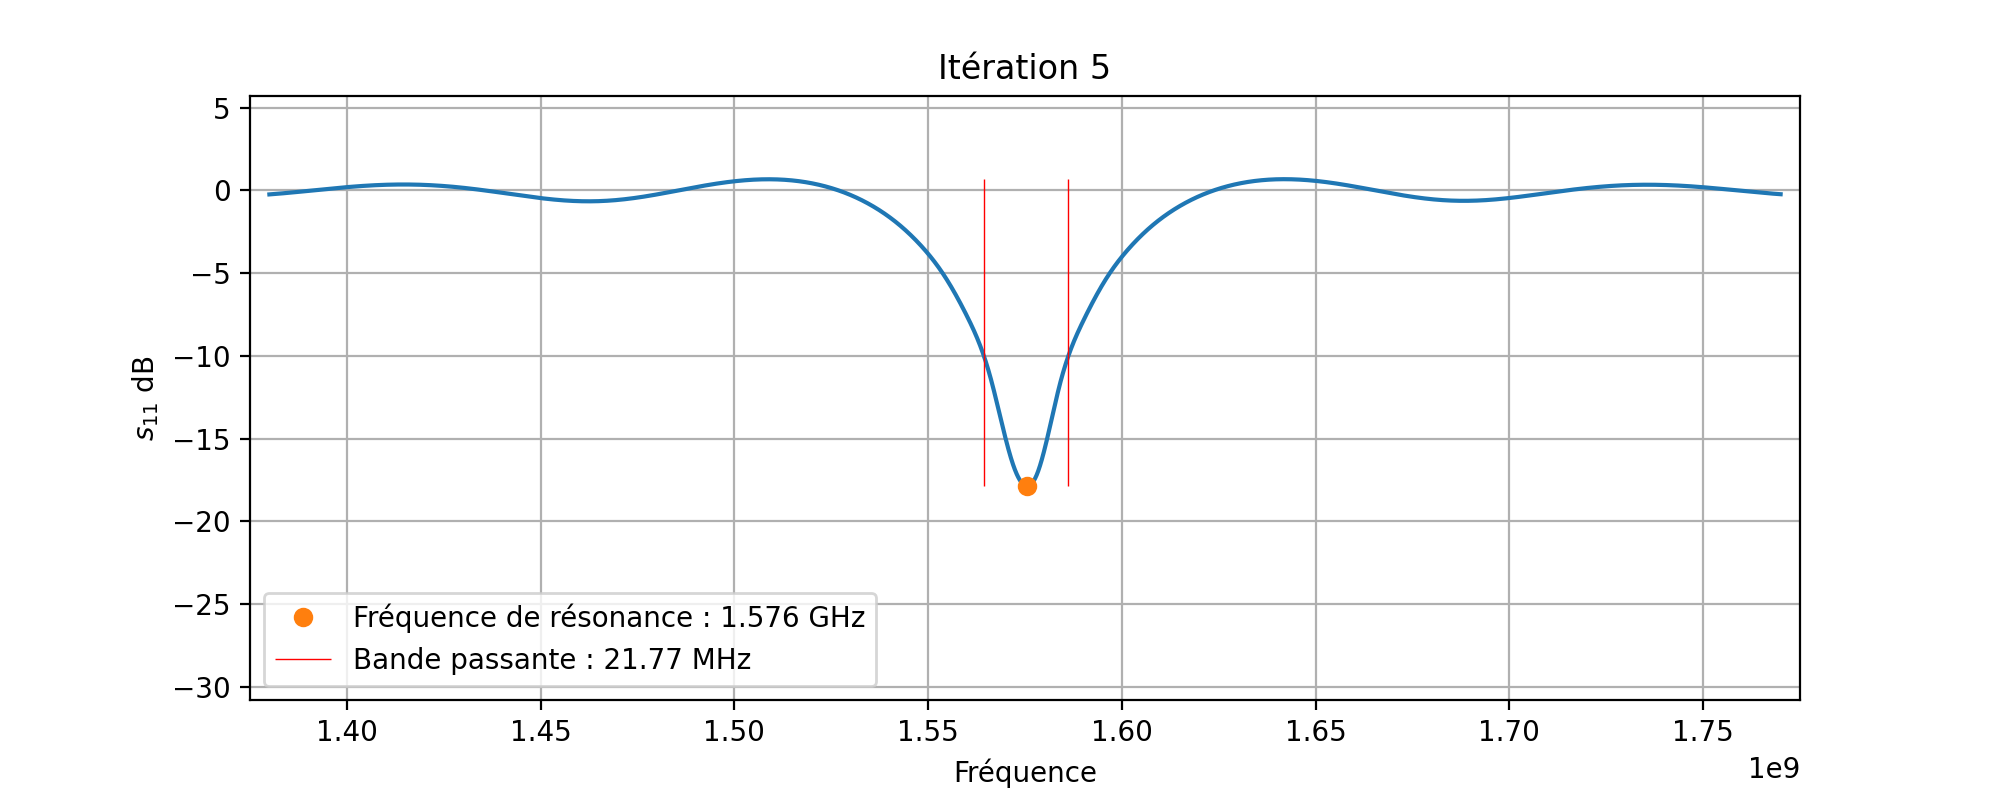
\includegraphics[width=15cm]{../Calculs/run_id_ceramique_5.png}
\caption[caption]{$s_{11}$ de l'itération 5}
\end{figure}
La fréquence de résonance est parfaite mais la bande passante n'est pas bonne.
\subsubsection{Sixième itération : Essai d'amélioration du $s_{11}$}
La dimension $y_0$ est diminuée à \SI{13}{\milli\meter}
\begin{figure}[H]
\centering
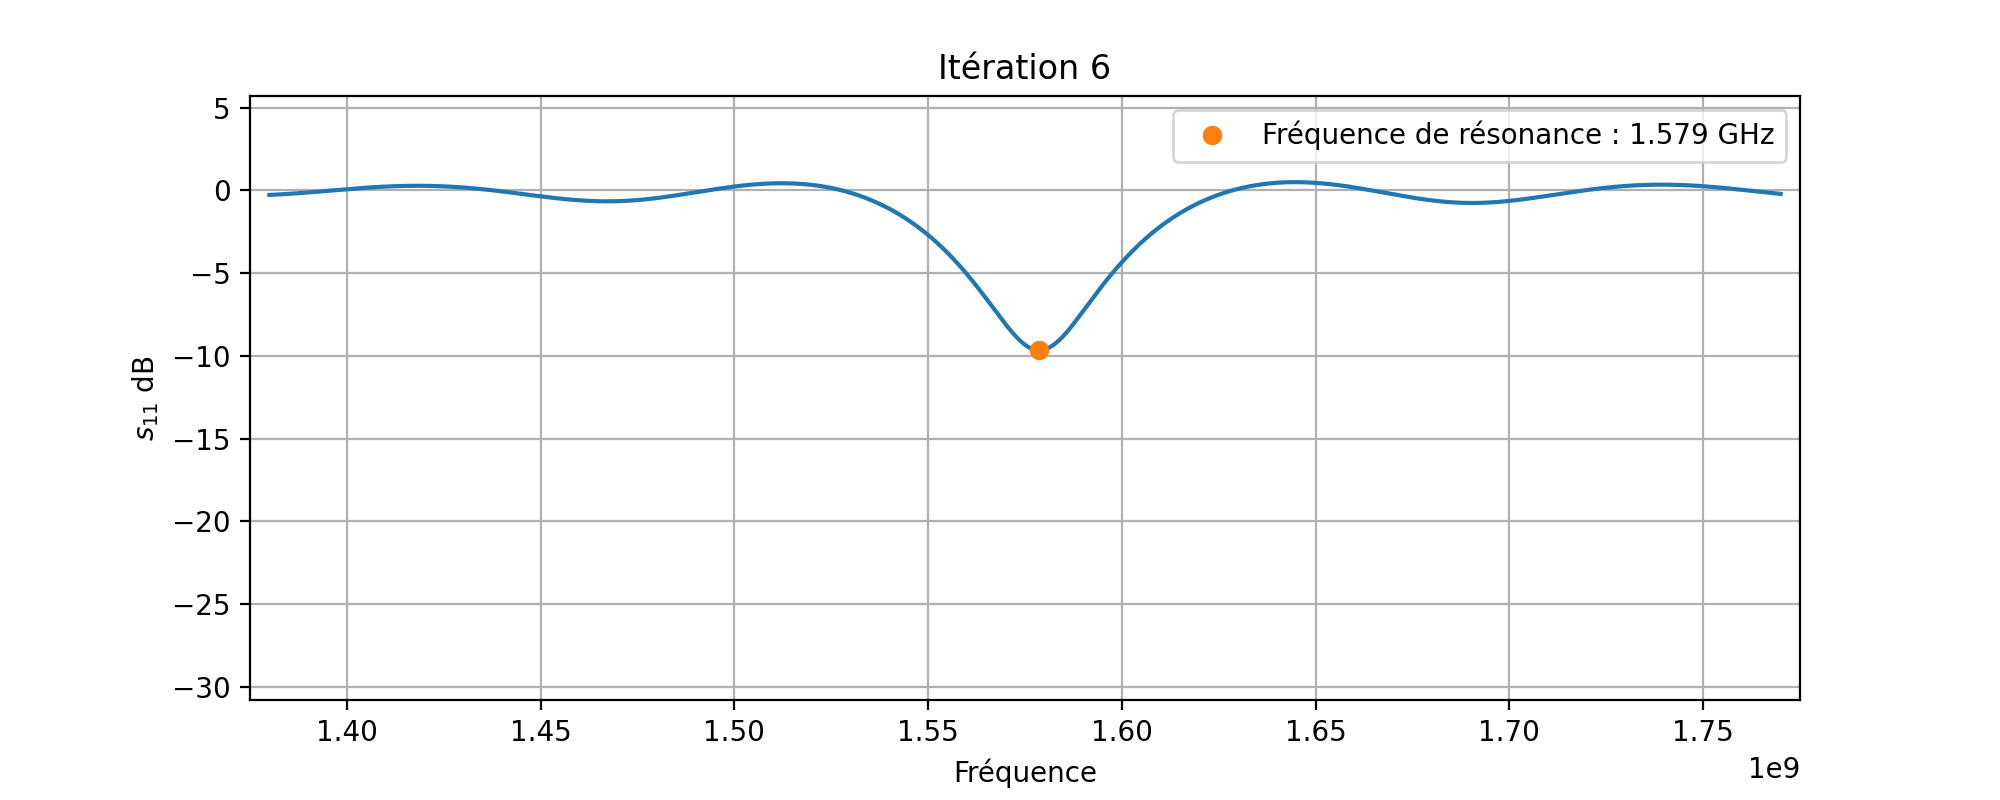
\includegraphics[width=15cm]{../Calculs/run_id_ceramique_6.png}
\caption[caption]{$s_{11}$ de l'itération 6}
\end{figure}
Le $s_{11}$ est moins bon qu'avant
\subsubsection{Septième itération : Essai d'amélioration du $s_{11}$}
La dimension $y_0$ est augmentée à \SI{17}{\milli\meter}
\begin{figure}[H]
\centering
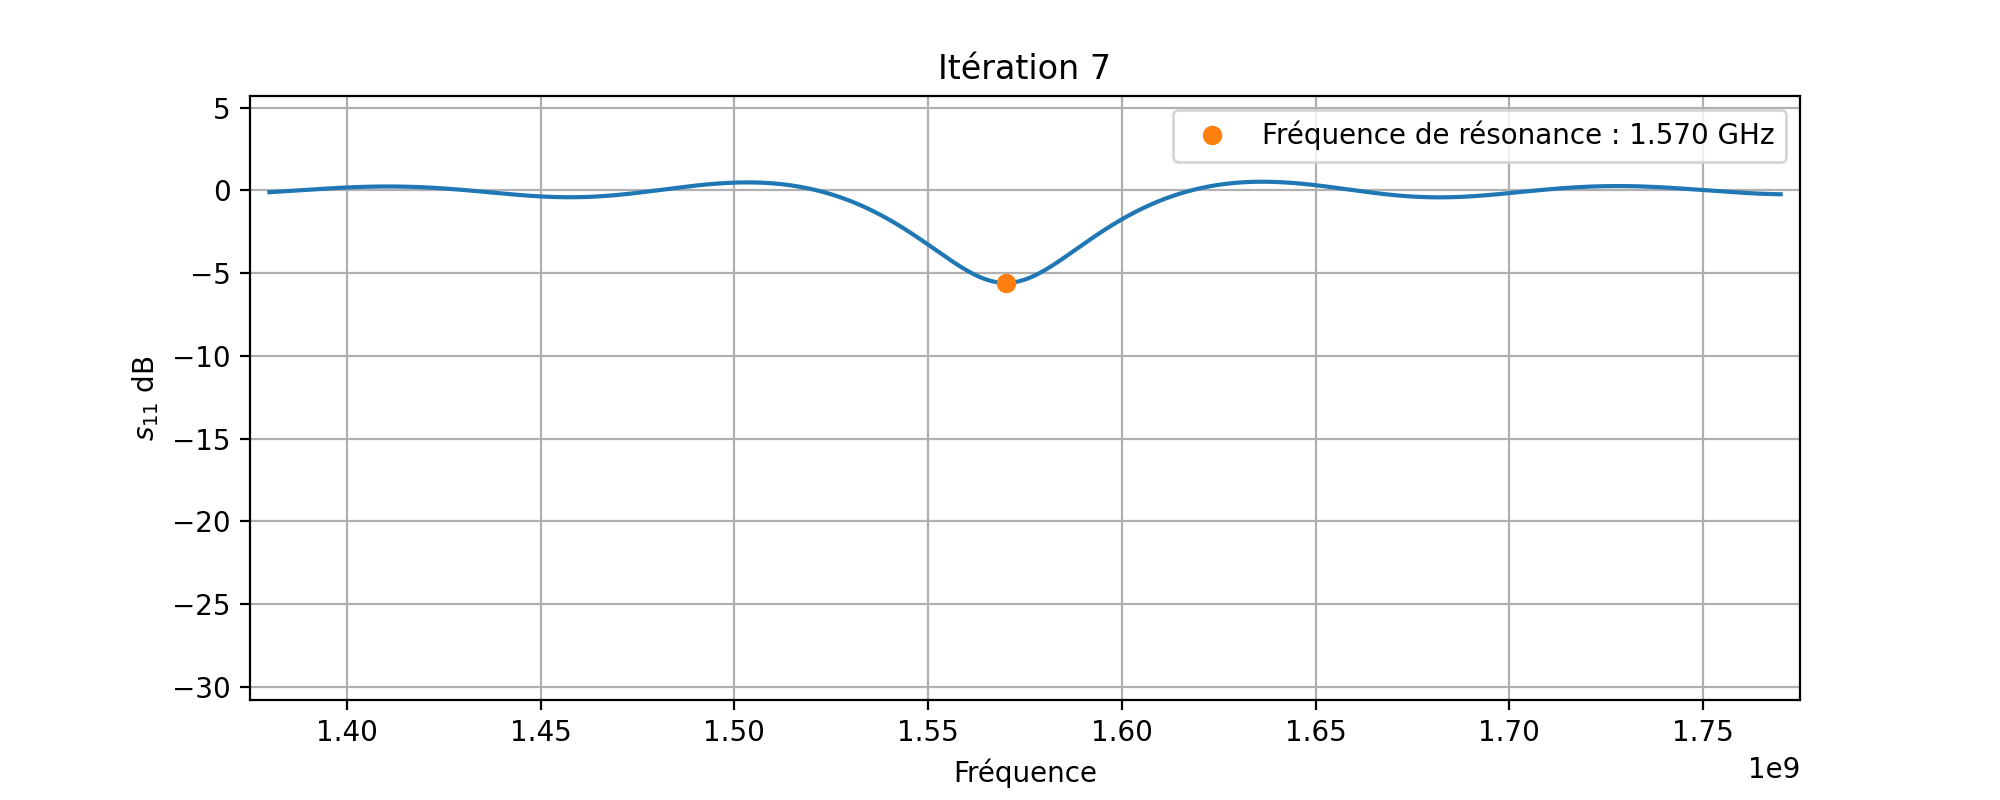
\includegraphics[width=15cm]{../Calculs/run_id_ceramique_7.png}
\caption[caption]{$s_{11}$ de l'itération 7}
\end{figure}
Le $s_{11}$ est moins bien qu'avant
\subsubsection{huitième itération : Essai d'amélioration du $s_{11}$}
Au lieu d'augmenter $y_0$, on le diminue à \SI{15}{\milli\meter}
\begin{figure}[H]
\centering
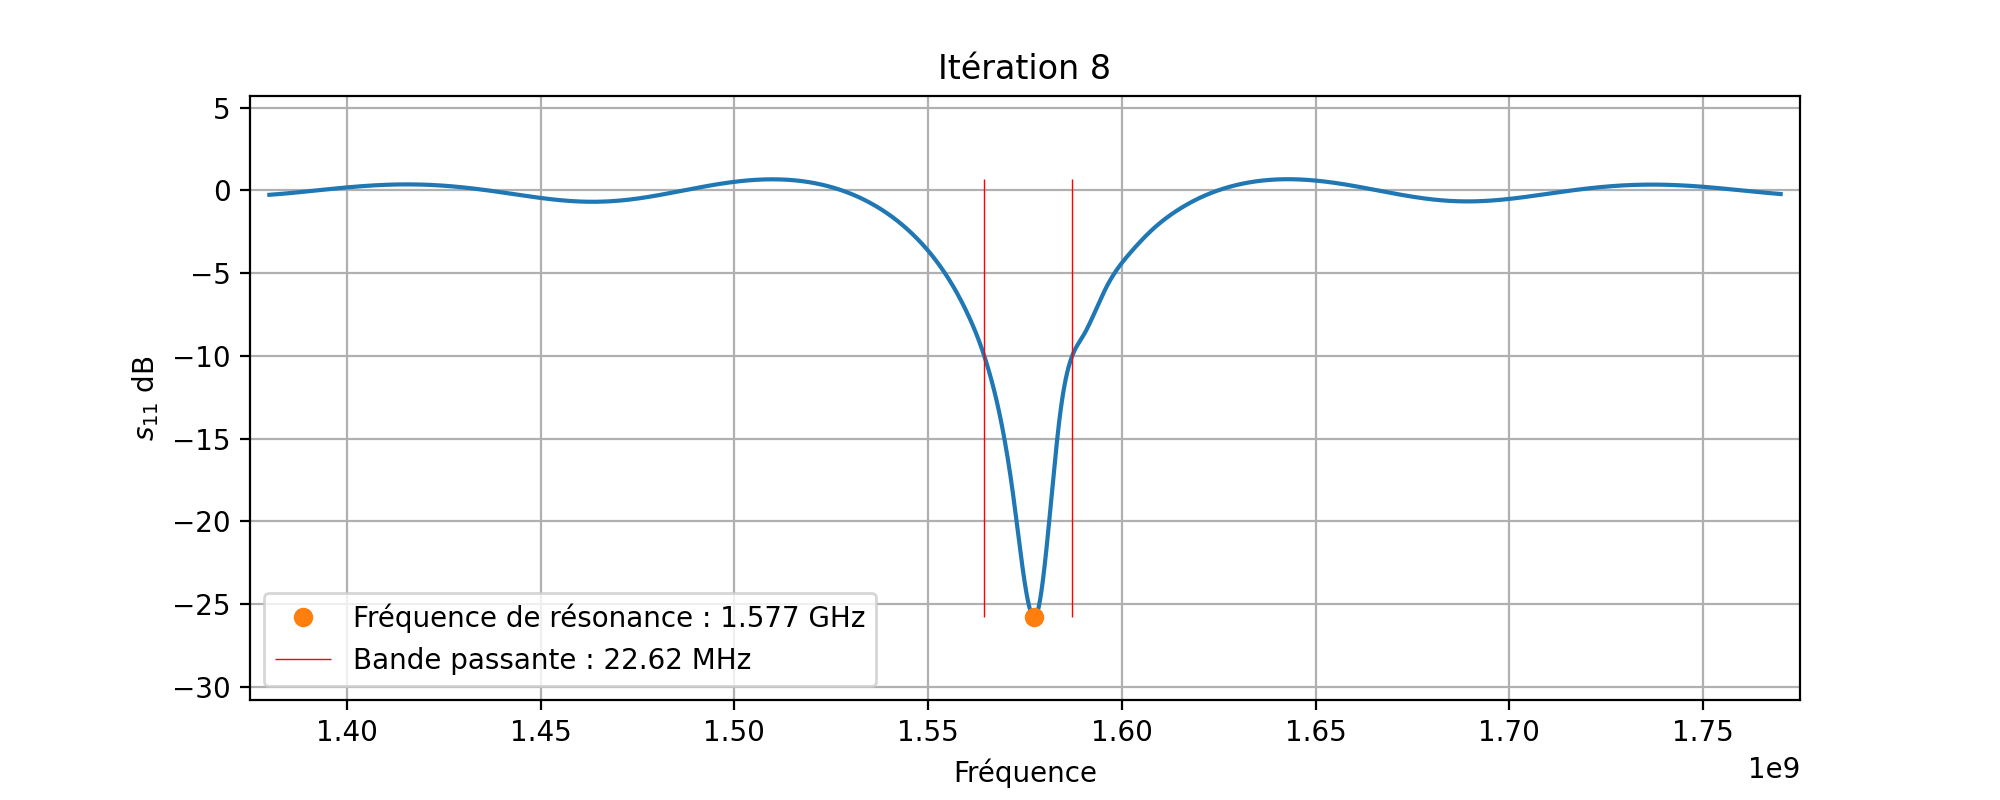
\includegraphics[width=15cm]{../Calculs/run_id_ceramique_8.png}
\caption[caption]{$s_{11}$ de l'itération 8}
\end{figure}
Le minimum de $s_{11}$ est très bon mais la bande passante n'est pas améliorée
\subsubsection{Neuvième et dixième itérations : Changement de l'épaisseur}
Par curiosité, nous avons modifié l'épaisseur du substrat pour étudier l'impact sur le $s_{11}$ (\SI{4}{\milli\meter} et \SI{3}{\milli\meter})
\begin{figure}[H]
\centering
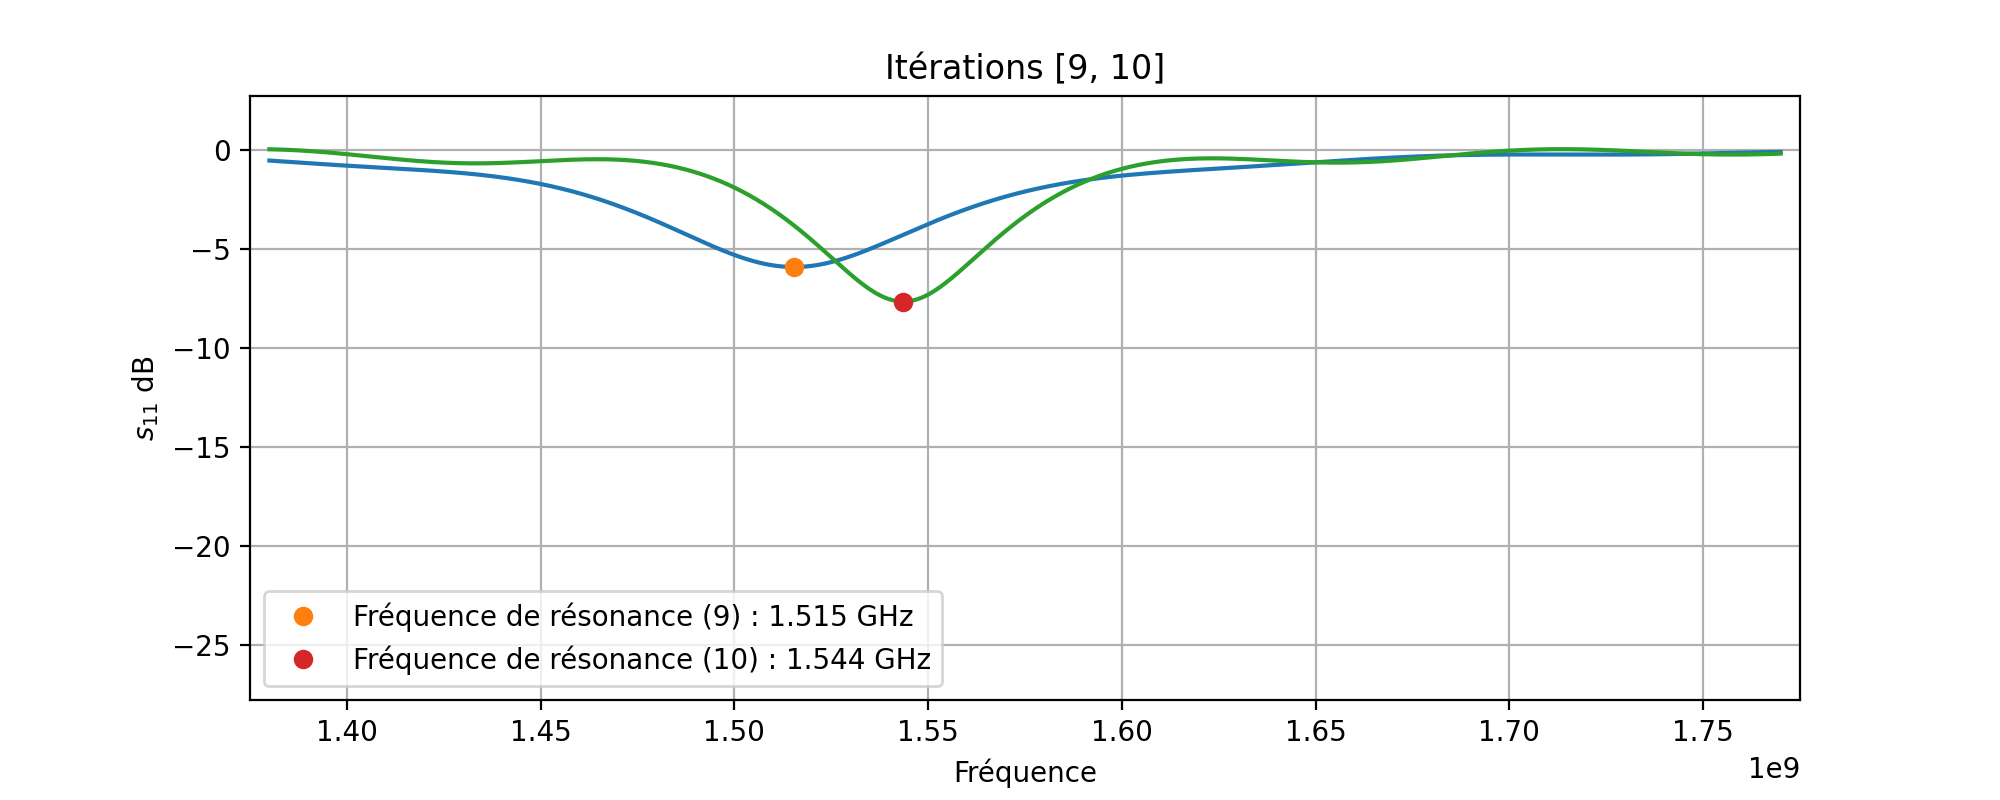
\includegraphics[width=15cm]{../Calculs/run_id_ceramique_910.png}
\caption[caption]{$s_{11}$ des itérations 9 et 10}
\end{figure}
L'impact de la modification de l'épaisseur est plutôt négatif. La modification des autres paramètres pourrait aider à améliorer le $s_{11}$.
\subsection{Conclusion}
Comme pour l'antenne FR-4, il est facile d'obtenir une bonne fréquence de résonance mais obtenir une bande passante acceptable est très difficile. La meilleure solution possède une fréquence de résonance de \SI{1.577}{\giga\hertz} et une bande passante de \SI{22.6}{\mega\hertz}. Les dimensions finales sont :
\begin{itemize}
\item $W=\SI{39.7}{\milli\meter}$
\item $L=\SI{30.57}{\milli\meter}$
\item $w_0=\SI{1.1}{\milli\meter}$
\item $y_1=\SI{23.79}{\milli\meter}$
\item $y_0=\SI{15}{\milli\meter}$
\end{itemize}
Dans l'ensemble nous avons l'impression que développer une antenne sur céramique est plus facile que sur FR-4. Il semblerait que ce fait soit connu car beaucoup d'antennes disponibles sur la marché (en format SMD) sont réalisées en céramique.







\end{document}